\documentclass[10pt,conference]{IEEEtran}

% ICSE 2027 Research Track requires IEEE conference proceedings format:
% \documentclass[10pt,conference]{IEEEtran}
% Do not use compsoc or compsocconf options.
% Review mode: double-anonymous; author block intentionally left blank.

\usepackage{cite}
\usepackage{amsmath,amssymb,amsfonts}
\usepackage{graphicx}
\usepackage{textcomp}
\usepackage{xcolor}
\usepackage{booktabs}
\usepackage{multirow}
\usepackage{array}
\usepackage{url}
\usepackage{xspace}
\usepackage{listings}
\usepackage[hidelinks]{hyperref}

\newif\ifshowrefs
\showrefstrue  % real \cite{} commands and refs.bib entries are present

% Source-compatible no-op helpers.
\newcommand{\todo}[1]{}
\newcommand{\ph}[1]{#1}
\newcommand{\figbox}[2]{}

% Short system-name macro so we can rename the tool in one place.
\newcommand{\sys}{\textsc{EvalTriage}\xspace}

% Abbreviation / enumerator macros (centralize house style).
\newcommand{\eg}{e.g.,\xspace}
\newcommand{\ie}{i.e.,\xspace}
\newcommand{\first}{(1)\xspace}
\newcommand{\second}{(2)\xspace}
\newcommand{\third}{(3)\xspace}
\newcommand{\fourth}{(4)\xspace}
\newcommand{\fifth}{(5)\xspace}
\newcommand{\RQ}[1]{\textbf{RQ#1}\xspace}

% Listing style for inline code snippets.
\lstset{
  basicstyle=\ttfamily\scriptsize,
  breaklines=true,
  columns=fullflexible,
  keepspaces=true,
  showstringspaces=false,
  numbers=none,
  frame=single,
  framesep=3pt,
  xleftmargin=2pt,
  aboveskip=4pt,
  belowskip=4pt,
}

\begin{document}

\title{EvalTriage: Diagnosing Evaluation Deviations in Embodied AI Pipelines
}

% Double-anonymous submission: omit author names and affiliations.
\author{}

\maketitle

\begin{abstract}
Embodied artificial intelligence (AI) systems are typically evaluated through benchmark pipelines that combine policies, checkpoints, simulators, task suites, reset states, interface adapters, seeds, and metric protocols. However, when an aggregate score changes, the available evidence is often insufficient to determine whether the deviation reflects a likely true regression, a setup-sensitive evaluation change, or an inconclusive outcome. This ambiguity limits the robustness and interpretability of embodied AI evaluation. This paper presents \sys, a factor-directed diagnosis framework for embodied AI evaluation deviations. \sys represents evaluation runs with structured manifests and episode-level outcomes, detects aggregate and paired-outcome deviations, and uses targeted differential replay to test factor-level hypotheses. It produces evidence-aware reports that classify deviation status, rank likely factors, and abstain when attribution is not sufficiently supported. We ground the problem through an empirical analysis of 473 GitHub issues and pull requests from 15 embodied AI and robot-learning projects, and evaluate \sys on a LeRobot--LIBERO artifact corpus covering completed rollouts, failed executions, calibration cases, ablations, robustness scenarios, and true-regression probes. \sys attributes all detected paper-only and robustness cases in our corpus to the expected factor, makes no false setup attributions on 12 negative calibration cases, and correctly classifies 66/67 main-status cases. Its factor-directed replay reduces diagnosis workload by 69.3\% compared with a blind rerun-$k$ baseline. These results show that embodied AI benchmarks can be made more reliable by complementing aggregate metrics with structured, factor-level diagnostic evidence.
\end{abstract}


\begin{IEEEkeywords}
software engineering for AI, embodied AI, robot learning, evaluation pipelines,
regression testing, reproducibility, differential replay, diagnosis
\end{IEEEkeywords}

\section{Introduction}
\label{sec:intro}

Embodied AI and robot-learning systems are typically evaluated through benchmark pipelines rather than through a model in isolation. A single run may depend on the policy checkpoint, simulator, task suite, reset state, controller semantics, observation preprocessing, dependency versions, seeds, and success definition. Prior work shows that reinforcement-learning results are sensitive to evaluation and experimental choices \cite{henderson2018drlmatters}; in embodied settings, those choices are embedded in larger evaluation pipelines. As a result, a changed success rate or episode outcome is often ambiguous: it may indicate a likely true policy regression, a setup-sensitive evaluation change, or evidence too weak to support attribution.

This ambiguity creates a practical diagnosis problem. Aggregate metrics can show that a benchmark result changed, but not why. Blind reruns can test repeatability, but do not identify whether the cause is a controller-interface mismatch, a changed reset state, an observation adapter, dependency drift, or a policy regression. Manifest differences identify changed fields, but a diff alone cannot establish causality. Interpreting embodied-AI evaluations therefore requires both structured provenance for candidate factors and behavioral or failure-recovery evidence to test them.

\sys addresses this problem by treating evaluation deviation diagnosis as a factor-directed evidence task. For baseline, current, and replay runs, it records structured manifests, summaries, episode outcomes, logs, and failure records when execution fails. It detects aggregate, paired-outcome, and failed-run deviations; maps manifest and failure differences to factor families such as action/controller interface, observation preprocessing, reset state, protocol/metric, dependency/runtime, checkpoint/config compatibility, and data format; and schedules targeted differential replays. These factors are hypotheses, not diagnoses. \sys attributes a setup-sensitive deviation only when replay or recovery evidence supports the factor, reports likely true regression when external-factor evidence does not explain a thresholded deviation, and returns unknown when the evidence is weak.

We ground the factor space through an empirical analysis of real project records. Across 15 embodied AI and robot-learning projects, keyword mining produced 2,714 candidate issues and pull requests, a relevance screen assisted by a large language model (LLM) retained 641, and manual classification retained 473 evidence records for the final taxonomy. We then evaluate \sys on a LeRobot--LIBERO artifact corpus covering completed rollouts, failed executions, calibration cases, ablations, robustness scenarios, and true-regression probes. \sys attributes all detected paper-only and robustness cases in our corpus to the expected factor, makes no false setup attributions on 12 negative calibration cases, classifies 66/67 main-status cases, and reduces diagnosis workload by 69.3\% compared with a blind rerun-$k$ baseline.

This paper makes the following contributions:
\begin{itemize}
  \item We frame embodied AI evaluation deviation diagnosis as an evidence-aware benchmark interpretation problem that complements aggregate metrics with evidence.
  \item We present a taxonomy of deviation symptoms and engineering factors from 473 GitHub issues and pull requests across 15 embodied AI and robot-learning projects.
  \item We introduce \sys, a manifest- and replay-based diagnosis technique for deviation detection, factor-directed replay, attribution, and abstention.
  \item We evaluate \sys on LeRobot+LIBERO artifacts spanning completed-rollout deviations, failed-run cases, negative calibration, ablations, robustness cases, true-regression probes, and replay-cost measurements.
\end{itemize}

\section{Motivating Example}
\label{sec:motivating-example}

Real project reports show why a changed embodied-AI benchmark score is not self-explanatory. In one LeRobot/LIBERO report, evaluating an X-VLA checkpoint on LIBERO-10 produced 0\% success until the evaluation was run with the absolute control mode expected by the checkpoint \cite{lerobot3401}. In another report, a converted pi0.5 LIBERO checkpoint evaluated at zero success despite a much higher reported reference number; the discussion pointed to image processing and normalization differences between pipelines \cite{lerobot2533}. Other reports involve the harness or runtime rather than a completed rollout: an evaluation bug unintentionally capped the number of unique LIBERO initial states sampled by \mbox{\emph{-{}-eval.batch\_size}} \cite{lerobot2850}, and a reset/lifecycle bug crashed evaluation after an environment was closed and later reused \cite{lerobot3814}. These examples have different observable symptoms, but they share the same diagnosis problem: the aggregate result does not identify which evaluation factor changed, whether the factor explains behavior, or whether the evidence is too weak to attribute.

Figure~\ref{fig:motivating-example} shows a controlled version of the action-interface pattern. We use a controlled case rather than a GitHub issue because diagnosis requires comparable baseline, current, and replay artifacts. The baseline evaluates the same policy on LIBERO-Goal tasks 0--9 with the expected relative action-control interface and obtains a success rate of 0.80. The current run changes the action control mode from relative to absolute and drops to 0.10. This drop alone is not enough to diagnose the cause: a rerun-$k$ or statistical gate can observe that results differ, but it cannot decide whether the change is a policy regression, a flaky run, or an evaluation-interface mismatch.

\begin{figure}[!b]
  \centering
  
\includegraphics[width=\columnwidth]{figures/fig1.pdf}
  \caption{Motivating diagnosis case: baseline and current runs first expose an action-control deviation, then a factor-directed replay restores the control setting and recovers the baseline success rate.}
  \label{fig:motivating-example}
\end{figure}

The replay run restores the baseline action-control setting while holding the policy, task suite, and seed fixed. Its success rate returns to 0.80, giving replay-supported evidence that the deviation is setup-sensitive and attributable to the action/controller interface. A manifest-only method could identify the changed control field but would not know whether it caused the observed behavior; a metric-only method could detect the drop but would not know what to test next. \sys connects the two by treating the manifest difference as a hypothesis and replay recovery as supporting evidence.

The same structure extends beyond this particular metric drop. For an observation-preprocessing mismatch, the replay would restore the expected image or state processing path. For a reset or harness failure, the current run may have no comparable success rate at all, so the diagnosis must use a failure record and a recovery replay. The example therefore illustrates three requirements that recur throughout the paper: preserve evaluation context, connect candidate factors to behavioral or failure-recovery evidence, and abstain when the artifacts do not support a defensible attribution.

\section{Background and Problem Definition}
\label{sec:background-problem}

\subsection{Embodied AI Evaluation Pipelines}

An embodied AI evaluation pipeline combines a learned policy with a simulator or robot environment, task definitions, reset states, observation and action adapters, dependency versions, and metric definitions. In our evaluation setting, LeRobot provides the evaluation harness and learned policy interface, while LIBERO provides manipulation task suites for robot-learning evaluation \cite{liu2023libero,lerobot2026}. Unlike a deterministic pass/fail unit test, a benchmark run produces aggregate metrics and episode-level traces that can vary across seeds, initial states, runtime environments, and protocol settings.

We use the term \emph{pipeline} deliberately. The measured behavior is not produced by the policy alone. Before an episode begins, the harness chooses a task, initializes a scene, resets the environment, loads a checkpoint and processor state, and configures observation and action adapters. During the episode, controller semantics and simulator state determine how the policy output is interpreted. After the episode, the benchmark turns observations and task conditions into a success label. A deviation can enter at any of these boundaries, so a diagnosis must preserve more context than the final success rate.

\subsection{Evaluation Deviations}

We define an \emph{evaluation deviation} as a statistically or semantically meaningful difference between a current evaluation and a baseline. Deviations include success-rate drops, reward or score mismatches, changed episode outcomes, rollout anomalies, crashes, and reproduction failures. We distinguish two observable classes. A \emph{completed-rollout deviation} has metrics and episode traces for the baseline and current run. A \emph{failed-run deviation} occurs when the evaluation itself crashes or fails before producing comparable rollout metrics.

The distinction between completed-rollout and failed-run deviations changes what evidence is available. In a completed rollout, diagnosis can compare aggregate success, task-level success, and paired episode outcomes. In a failed run, the current artifact may contain no comparable task metric, but the failure record and point of failure can identify a factor family. \sys therefore avoids a single metric-only definition of deviation. It treats metric drops, paired-outcome shifts, and evaluation failures as different observable symptoms of the same diagnosis task. Figure~\ref{fig:problem-anatomy} summarizes this anatomy.

\begin{figure}[!t]
  \centering
  
\includegraphics[width=\columnwidth]{figures/fig2.pdf}
  \caption{Problem anatomy for embodied-AI evaluation deviation diagnosis: metric drops, paired episode shifts, and failed runs are symptoms that must be connected to manifest, failure-record, and replay evidence before \sys attributes a status or abstains.}
  \label{fig:problem-anatomy}
\end{figure}

\subsection{Diagnosis Task}

An instance of the diagnosis task consists of a baseline run artifact $A_b$, a current run artifact $A_c$, and optional replay artifacts $A_r$. Each artifact may contain a manifest, aggregate summary, episode-level outcomes, logs, cost records, and, for failures, a failure record. The task is not to score a policy. It is to explain a comparison: why does $A_c$ differ from $A_b$, and what evidence supports or blocks attribution?

We formalize the desired output as a triple
$(s,\rho,E)$. The status $s$ is one of four evidence states:
\emph{setup-sensitive deviation}, \emph{likely true regression},
\emph{unknown}, or \emph{flaky evaluation} when repeated-run evidence is
available. The ranking $\rho$ is an ordered list of candidate factor
families only when the evidence supports attribution. The evidence record
$E$ summarizes the observed symptom, relevant manifest or failure-record
differences, replay outcomes, affected tasks or episodes, and any missing
evidence that prevents a stronger conclusion.

The central constraint is that a factor difference is only a hypothesis. A
manifest diff may show that the control mode, reset configuration, camera
pipeline, dependency version, checkpoint metadata, or metric protocol
changed, but that diff is not itself a diagnosis. A setup-sensitive
diagnosis requires behavioral or failure-recovery evidence: controlling or
restoring the suspected factor must recover baseline behavior, explain the
failed run, or otherwise connect the factor to the observed symptom. A
likely true regression is reported only when the deviation remains after external
evaluation factors have been controlled and the remaining evidence points
to the policy or semantic code change. If no thresholded deviation is
detected, if replay evidence conflicts, or if the needed artifacts are
missing, the correct output is unknown rather than a forced factor.

This definition separates diagnosis from three adjacent tasks. It is not
performance improvement: \sys does not train a better policy, propose a new
benchmark, or decide whether a policy is good. It is not experiment logging:
logging records what changed, whereas diagnosis asks whether that change
explains the observed behavior. It is also not generic flaky-test detection:
instability is reported only when comparable repeated runs support it.
The task is therefore evidence-governed attribution: produce a factor-level
explanation when the artifacts justify one, and make the missing evidence
explicit when they do not.

\subsection{Engineering Factors}

The factors considered by \sys include seed/randomness, reset or initial state, simulator and runtime environment, dependency drift, action/controller interface, observation/sensor preprocessing, checkpoint/config compatibility, evaluation protocol/metric, evaluation harness behavior, data format, and semantic code regression. A factor is \emph{attributable} only when the evidence links it to the observed deviation; a manifest difference by itself is a suspect, not a diagnosis.

The factor vocabulary is intentionally engineering-facing. A developer can act on ``action/controller interface'' by checking controller mode and postprocessing, on ``checkpoint/config compatibility'' by inspecting processor state and checkpoint metadata, and on ``evaluation protocol/metric'' by reviewing task lists, episode lengths, thresholds, and success definitions. This vocabulary makes the diagnosis report closer to a debugging artifact than to a high-level model evaluation summary.

\subsection{Diagnosis Statuses}

\sys's primary statuses are setup-sensitive deviation, likely true regression, and unknown. A \emph{setup-sensitive deviation} is supported when controlling a changed engineering factor recovers baseline behavior. A \emph{likely true regression} is supported when external-factor replays fail to explain the deviation and semantic code or policy changes remain plausible. \emph{Unknown} is returned when no thresholded deviation is detected or when evidence is missing, weak, or conflicting. \sys can also report \emph{flaky evaluation} when comparable repeated runs vary without a stable factor explanation, but this status requires repeated-run instability evidence.

The statuses are ordered by evidential responsibility rather than by severity. A setup-sensitive deviation is not necessarily less serious than a likely true regression; it may still block a release if the benchmark protocol changed unintentionally. Similarly, unknown is not a failure to produce text. It is the appropriate outcome when the artifacts do not support a defensible explanation. This ordering prevents \sys from turning every detected difference into a confident diagnosis.

\section{Empirical Study of Evaluation Deviations}
\label{sec:empirical-study}

\subsection{Study Goal and Scope}

This empirical study characterizes the evaluation deviations and evaluation-affecting engineering factors reported in embodied AI and robot-learning projects. We study GitHub issues and pull requests as project-maintenance evidence of evaluation problems. These records capture developer-observed symptoms such as success-rate mismatches, rollout anomalies, evaluation crashes, reproduction failures, and unexpected benchmark behavior, together with suspected causes such as controller interfaces, reset states, simulator or runtime dependencies, checkpoint compatibility, observation preprocessing, and evaluation harness changes.

The goal of this study is to characterize the problem space rather than to estimate the prevalence of all embodied-AI bugs. Following empirical bug-study practice, we treat each retained record as evidence for a deviation symptom, an evaluation-affecting factor, an affected pipeline phase, and the strength of the explanatory evidence. This produces a taxonomy of symptoms and factors grounded in real project maintenance, and it also identifies the kinds of artifacts that a diagnosis method must explicitly reason about: manifests, run outcomes, episode-level behavior, failed executions, and cases where the available evidence is insufficient for attribution.

\subsection{Data Collection and Classification}

We mined GitHub issues and pull requests from 15 embodied-AI and robot-learning projects, including LeRobot, LIBERO, ManiSkill, Habitat-Sim, Habitat-Lab, ManiSkill-Learn, RLBench, robosuite, MetaWorld, CALVIN, OpenVLA, OFT, vla-evaluation-harness, Isaac Lab, and SimplerEnv. Keyword mining produced 2,714 candidates. A relevance screen assisted by a large language model retained 641 candidates about evaluation, benchmarking, rollout behavior, reproducibility, or evaluation-affecting factors. We then manually classified the screened candidates and retained 473 evidence records for the final taxonomy. The frozen JSON Lines (JSONL) record keeps the original repository, URL, issue or pull-request text, comments, matched keywords, human classification fields, and short evidence quotes.

Each retained record is classified by four dimensions: evidence role, primary deviation symptom, primary engineering factor, and affected pipeline phase. Evidence role records whether the report contains both a deviation and an explanatory factor, only a deviation, or only a factor that can plausibly change evaluation behavior. A single annotator manually classified the screened candidates, and the frozen records were then summarized deterministically; we use the study as problem evidence and taxonomy construction, not as a precise prevalence estimate over all embodied-AI maintenance.

The classification intentionally uses project-maintenance language rather than model-centric language. For example, an issue that reports a crash during reset is classified as an evaluation crash or failure, with reset or initial state as the factor if the thread identifies stale environment state as the cause. A pull request that changes controller semantics is classified by the action/controller interface factor even if it does not report a specific metric drop. This coding scheme preserves the engineering context that developers use when they triage benchmark changes and provides the factor vocabulary for the controlled evaluation matrix.

\begin{table}[!t]
  \caption{RQ1 Evidence Summary}
  \label{tab:rq1-summary}
  \centering
  \renewcommand{\arraystretch}{1.10}
  \begin{tabular}{lrr}
    \toprule
    Evidence role & Count & Percent \\
    \midrule
    Deviation and factor & 258 & 54.55\% \\
    Deviation only & 144 & 30.44\% \\
    Factor only & 71 & 15.01\% \\
    \midrule
    Total & 473 & 100.00\% \\
    \bottomrule
  \end{tabular}
\end{table}

\begin{figure}[t]
  \centering
  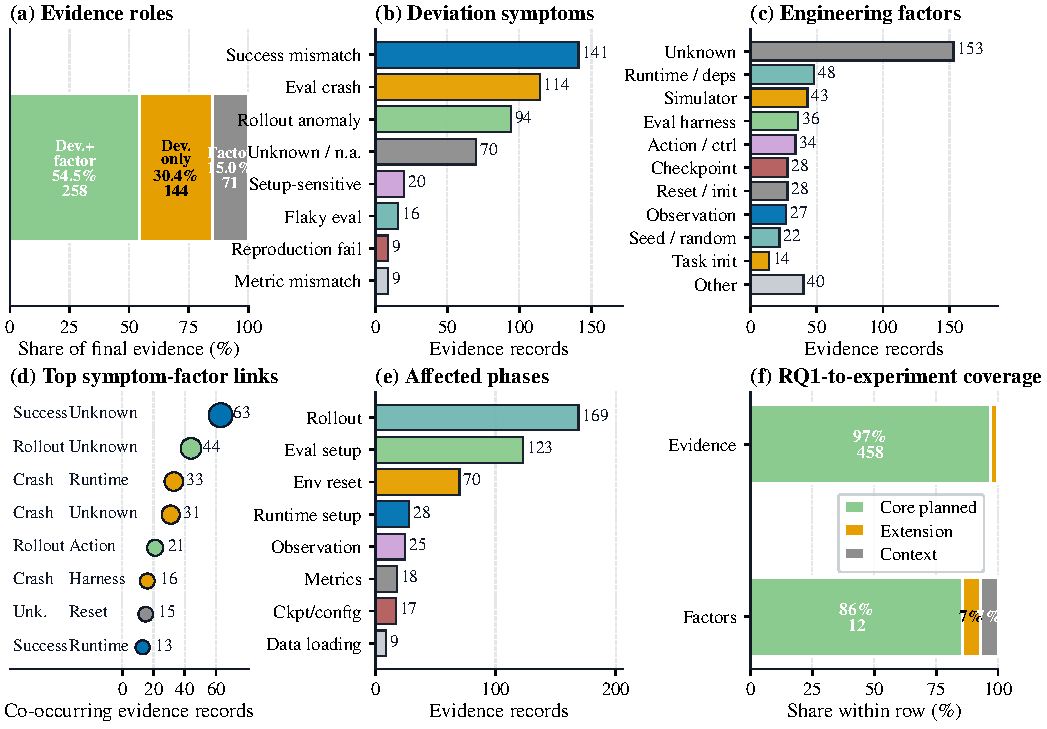
\includegraphics[width=\columnwidth]{figures/rq1_evidence_overview.pdf}
  \caption{RQ1 evidence overview: the panels summarize evidence roles, deviation symptoms, engineering factors, symptom--factor links, affected pipeline phases, and how the taxonomy maps to the controlled evaluation coverage.}
  \label{fig:rq1-evidence}
\end{figure}

\subsection{Results}

\noindent\textbf{Deviation symptoms.}
Figure~\ref{fig:rq1-evidence} and Table~\ref{tab:rq1-summary} show that evaluation deviations are not confined to one symptom type. Success-rate drops or mismatches account for 141 records, evaluation crashes or failures for 114 records, and rollout behavior anomalies for 94 records. The remaining records include setup-sensitive outcomes, instability or flakiness reports, reward/score mismatches, and reproduction failures. These categories span completed rollouts, failed executions, and reproduction problems, rather than a single aggregate metric.

\noindent\textbf{Finding~1.} Evaluation deviations are heterogeneous: real reports include aggregate metric changes, rollout anomalies, execution failures, and reproduction gaps.

\noindent\textbf{Engineering factors.}
The largest specified factor families include dependency/runtime environment, simulator/physics/rendering, evaluation script or harness behavior, action/controller interface, checkpoint/config compatibility, reset or initial state, and observation/sensor preprocessing. These factors often sit outside the learned policy itself. A changed benchmark result can therefore be associated with the evaluation stack, the task wrapper, or the controller interface even when the checkpoint is unchanged.

\noindent\textbf{Finding~2.} Many reported deviations are tied to evaluation-stack factors rather than to the policy checkpoint alone.

\noindent\textbf{Underspecified evidence.}
The factor \mbox{\emph{unknown\_or\_not\_specified}} appears in 153 of 473 records, or 32.35\%. These records often report a symptom without a confirmed causal factor, or mention configuration differences without enough behavioral evidence for causal attribution. This under-specification is part of the empirical phenomenon rather than an annotation error: project threads frequently stop after a workaround, reproduction gap, or partial diagnosis.

\noindent\textbf{Finding~3.} A substantial fraction of real reports lacks enough evidence for confident factor attribution.

\subsection{Implications for Controlled Evaluation}

These empirical observations shape the controlled LeRobot+LIBERO matrix in three ways. First, the matrix must include both completed-rollout and failed-run cases, because real reports include both metric deviations and execution failures. Second, the factor set must span the evaluation pipeline rather than focusing only on seed changes or policy checkpoints. Third, the evaluation must include negative calibration cases, because real project records often contain configuration differences that are not sufficient evidence for causal attribution. These implications determine the later RQ3 denominator split between paper-only cases, failed-run cases, negative calibration cases, and robustness cases.

\section{Design of EvalTriage}
\label{sec:approach}

Figure~\ref{fig:approach-overview} shows the \sys workflow from run artifacts to evidence extraction, candidate factors, controlled replay, and diagnosis output.

\begin{figure*}[!t]
  \centering
  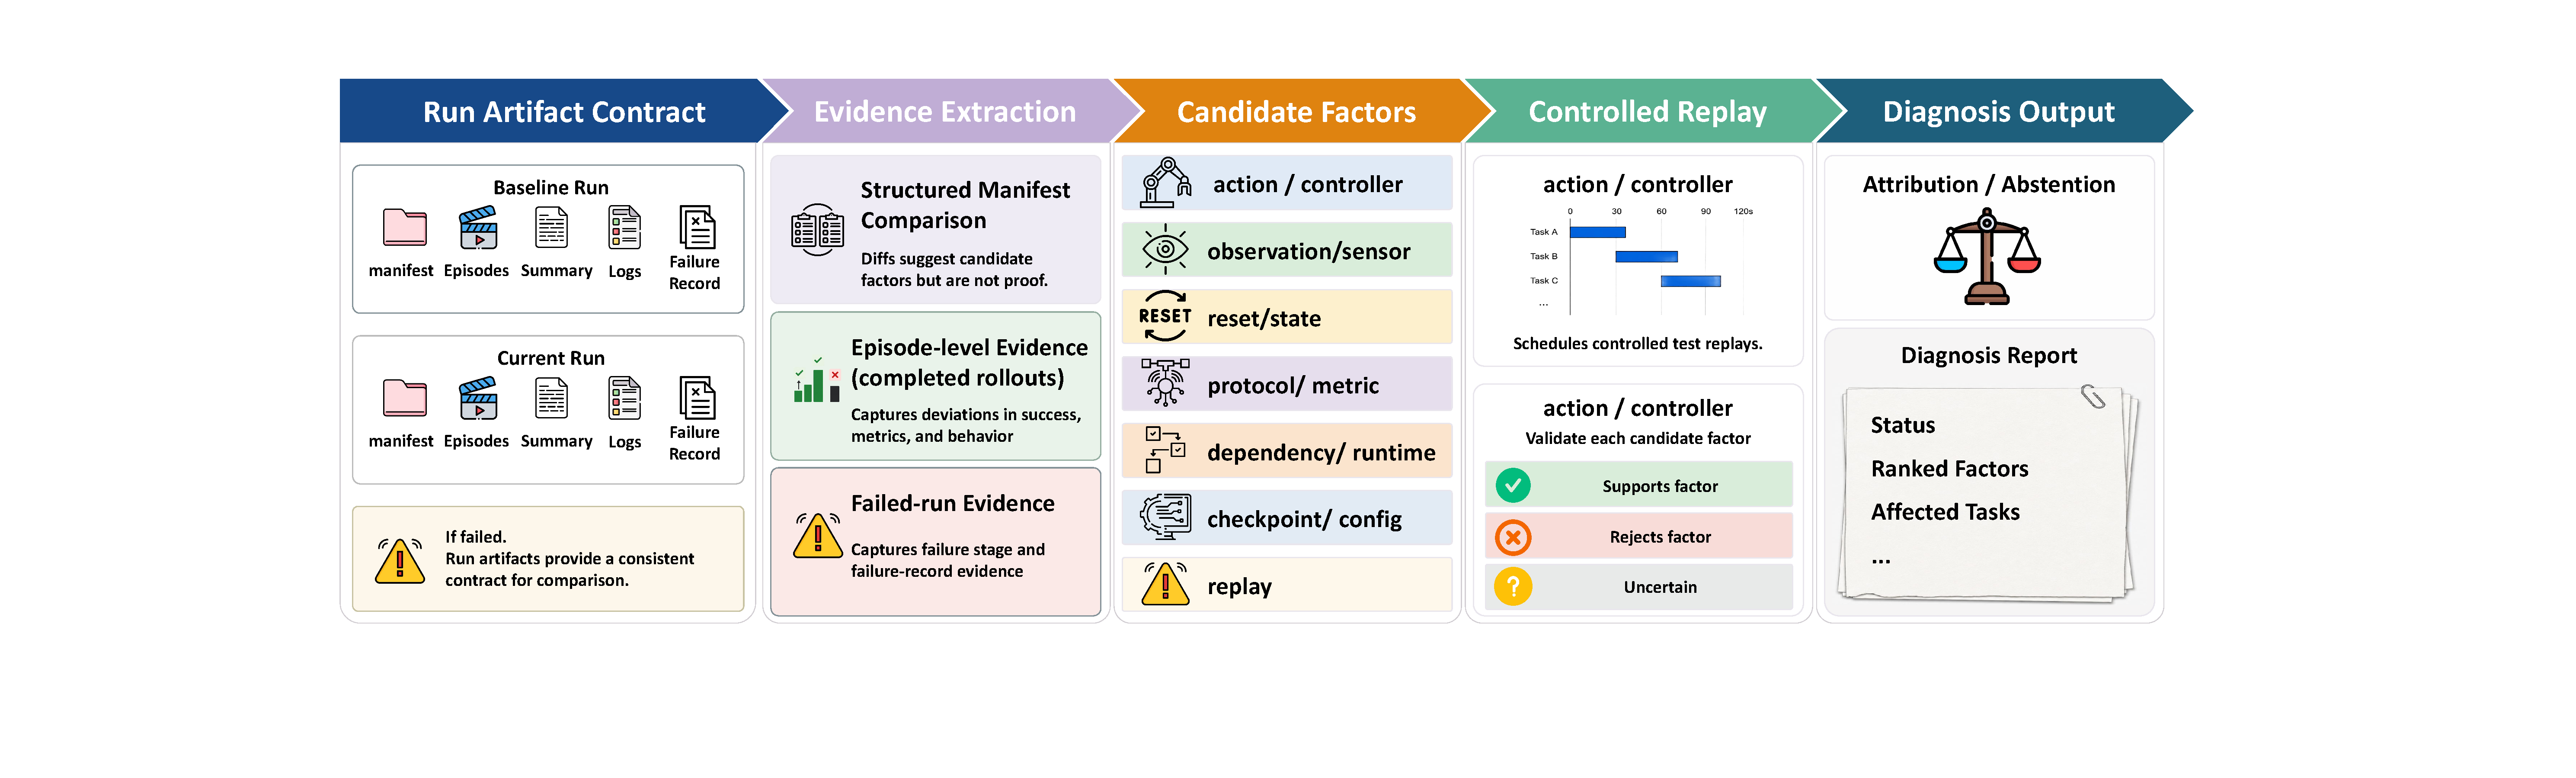
\includegraphics[width=\textwidth]{figures/fig4.pdf}
  \caption{\sys architecture: the workflow records baseline/current artifacts, extracts manifest, episode-level, and failed-run evidence, proposes candidate factors, validates them with controlled replay, and returns attribution or abstention.}
  \label{fig:approach-overview}
\end{figure*}

\subsection{Evaluation Manifest}

Each run produces a manifest that records the policy checkpoint, code version, runtime environment, task suite, seeds, evaluation protocol, observation preprocessing, action interface, reset configuration, metrics, and cost. Its fields define the candidate explanations that \sys can test. In controlled experiments, expected-factor labels and operator names are evaluation metadata, not diagnosis inputs: \sys consumes only run artifacts, manifest differences, failure records, episode outcomes, and replay outcomes, and labels are consulted only after a diagnosis is produced.

Table~\ref{tab:manifest-factors} shows how manifest fields map to factor families. The mapping is deliberately coarse enough to remain stable across projects, but concrete enough to guide replay. For example, a change in \mbox{\emph{action.control\_mode}} maps to the action/controller interface factor and can be tested by replaying with the baseline control mode. A change in task list, episode horizon, or success threshold maps to evaluation protocol/metric and can be tested by replaying the current policy under the baseline protocol. A missing processor statistic maps to checkpoint/config compatibility or observation preprocessing, depending on where the failure is observed.

\begin{table}[!t]
  \caption{Manifest Fields and Candidate Factors}
  \label{tab:manifest-factors}
  \centering
  \footnotesize
  \renewcommand{\arraystretch}{1.08}
  \begin{tabular}{@{}lp{0.56\columnwidth}@{}}
    \toprule
    Factor family & Representative manifest evidence \\
    \midrule
    Action/controller & Control mode, action scaling, postprocessing \\
    Observation/sensor & State keys, image transforms, processor stats \\
    Reset/state & Seeds, initial states, scene/task initialization \\
    Protocol/metric & Task list, episode length, success definition \\
    Dependency/runtime & Package versions, simulator backend, device \\
    Checkpoint/config & Policy checkpoint, processor, model config \\
    \bottomrule
  \end{tabular}
\end{table}

\subsection{Deviation Detection}

\sys detects deviations using aggregate metrics, failed-run status, and paired episode outcome shifts. Aggregate checks capture success-rate or reward changes. Failed-run checks capture crashes and preflight failures. Paired episode checks compare task/seed outcomes, which is important when the aggregate success rate is unchanged but the current run succeeds and fails on different episodes than the baseline.

The detector produces an evidence record rather than a binary pass/fail decision. For completed rollouts, the record includes baseline and current success rates, affected tasks, and paired episode changes. For failed runs, it includes the failing stage and the structured failure type. This record becomes the guard for attribution: if the detector does not find a thresholded deviation, \sys may still report manifest differences, but it cannot promote them to causal factors.

\subsection{Factor-Directed Replay}

Instead of blindly rerunning the benchmark, \sys plans replays that restore or control suspected factors. A replay may restore the action interface, observation pipeline, checkpoint configuration, evaluation protocol, runtime environment, dataset format, or reset behavior. The replay budget is intentionally small and targeted: it should test the most plausible factor explanation before developers repeat the benchmark.

Replay planning follows two principles. First, it preserves the comparison as much as possible: the policy, task suite, and seed remain fixed unless the suspected factor itself is one of those fields. Second, it changes only the factor being tested. This makes replay evidence interpretable. If a replay restores baseline behavior after restoring a controller interface, the controller interface becomes a supported explanation. If the replay does not recover, \sys should either try another supported factor or abstain rather than blame the most visible manifest diff without sufficient behavioral evidence.

The same idea applies to failed-run cases. A failed run may not have a success-rate drop because it does not finish. In that setting, a replay is successful when the run progresses past the failure and produces comparable artifacts. The diagnosis is therefore supported by failure recovery rather than metric recovery. This distinction is why failed-run cases are reported separately in the evaluation.

Operationally, \sys first identifies a completed-rollout or failed-run deviation, maps manifest or failure-record differences to candidate factors, and schedules a replay that tests the most plausible explanation.

\subsection{Diagnosis Rules}

\sys treats manifest and failure-record differences as hypotheses, not conclusions. A setup-sensitive attribution requires three pieces of evidence: a detected deviation, a candidate factor supported by manifest or failure evidence, and replay behavior that recovers baseline behavior or controls the failure. A factor with manifest evidence but no detected deviation is not eligible for attribution. A factor with deviation and manifest evidence but no replay support can appear as a candidate, but the diagnosis status remains unknown unless the artifact explicitly records the missing-evidence condition.

The same rules define abstention. If replay outcomes conflict, affected tasks are unstable across comparable runs, or critical artifacts are missing, \sys returns unknown rather than promoting the most visible manifest difference. This conservative rule is central to negative calibration and separates \sys from manifest-diff heuristics. Table~\ref{tab:diagnosis-statuses} lists the status vocabulary.

\begin{table}[!t]
  \caption{Diagnosis Statuses}
  \label{tab:diagnosis-statuses}
  \centering
  \renewcommand{\arraystretch}{1.08}
  \begin{tabular}{@{}p{0.30\columnwidth}p{0.64\columnwidth}@{}}
    \toprule
    Status & Meaning \\
    \midrule
    Setup-sensitive & A factor change explains the deviation through replay evidence. \\
    Flaky & Repeated comparable runs vary without a supported factor attribution. \\
    Likely true regression & Semantic code evidence remains after external-factor replays fail to explain the deviation. \\
    Unknown & Evidence is missing, weak, conflicting, or no thresholded deviation is detected. \\
    \bottomrule
  \end{tabular}
\end{table}

\subsection{Report and Artifact Contract}

The final report summarizes the affected task set, baseline/current/replay metrics, suspected factor ranking, supporting evidence, missing information, and recommended developer actions. It is meant to be inspected by developers, not only consumed as an aggregate score: a setup-sensitive report points to the recovered replay and the controlled manifest field, while an unknown report explains whether uncertainty comes from no detected deviation, missing replay, conflicting replay, or insufficient failure evidence.

\sys relies on a small file-based artifact contract between the evaluation harness and the diagnosis layer. A completed run provides a manifest, episode records, a summary file, and logs. A failed run additionally provides a failure record that states the failing stage and the exception or preflight condition. Replay runs use the same contract, which keeps baseline, current, and replay artifacts comparable and prevents diagnosis from depending on hidden process state. Table~\ref{tab:report-fields} shows the artifact fields that make the report auditable rather than purely textual.

\begin{table}[!t]
  \caption{Diagnosis Report Fields}
  \label{tab:report-fields}
  \centering
  \footnotesize
  \renewcommand{\arraystretch}{1.08}
  \begin{tabular}{@{}lp{0.60\columnwidth}@{}}
    \toprule
    Field & Purpose \\
    \midrule
    Status & Setup-sensitive, likely true regression, unknown; flaky only with repeat evidence \\
    Factor ranking & Top candidate factors and supporting evidence \\
    Affected tasks & Tasks or episodes whose outcomes changed \\
    Replay evidence & Recovery, non-recovery, or missing replay state \\
    Missing evidence & Reason for abstention or reduced confidence \\
    Cost & Episodes, reruns, graphics processing unit (GPU) minutes, and wall-clock minutes \\
    \bottomrule
  \end{tabular}
\end{table}

\section{Evaluation}
\label{sec:evaluation}

We evaluate \sys around four research questions:

\begin{itemize}
  \item[\textit{RQ1}] \textit{(Problem evidence)} Do real embodied AI projects contain evaluation deviations and evaluation-affecting factors that justify a dedicated diagnosis task?
  \item[\textit{RQ2}] \textit{(Status classification)} Can \sys distinguish setup-sensitive deviations, likely true regressions, and unknown evidence states?
  \item[\textit{RQ3}] \textit{(Factor attribution and abstention)} When a deviation is detected, can \sys identify the responsible engineering factor, and can it abstain on non-deviating calibration cases?
  \item[\textit{RQ4}] \textit{(Diagnosis cost)} How much execution cost does factor-directed diagnosis require relative to the evidence it provides?
\end{itemize}

\subsection{Experimental Setup}
\label{sub:eval-setup}

\noindent\textbf{Benchmark stack.} The controlled experiments use LeRobot+LIBERO with the \mbox{\emph{pi0\_libero\_finetuned\_v044}} policy. A case consists of a baseline run, a current run, and zero or more replay runs. Each completed-run artifact records \mbox{\emph{manifest.json}}, \mbox{\emph{episodes.jsonl}}, \mbox{\emph{summary.json}}, and \mbox{\emph{logs.txt}}. Failed-run artifacts additionally record \mbox{\emph{failure.json}}. This artifact interface is important because \sys is not allowed to infer a factor from prose notes alone: every diagnosis must trace to structured artifacts, replay evidence, or a declared missing-evidence condition.

\noindent\textbf{Ground-truth isolation.} The cases are controlled, but the evaluator and the diagnosis engine use different information. Case configurations contain expected factors for scoring, while \sys consumes only baseline/current/replay artifacts. The aggregation scripts compare the produced diagnosis against the expected factor after the report is written. This separation matters because otherwise a controlled case would risk testing whether the system can read an injected label rather than whether it can diagnose from behavior and replay evidence.

\noindent\textbf{Realism and control.} The controlled cases are not toy outputs or synthetic summaries. Each case executes the LeRobot+LIBERO stack and writes the same artifact contract used by the diagnosis pipeline. Control enters at the factor level: we choose one evaluation-affecting change, run the corresponding baseline/current/replay artifacts, and then check whether the diagnosis recovers the expected factor from artifacts alone. This design gives the experiment a causal oracle without relying on naturally occurring histories whose true cause may be undocumented. RQ1 supplies the empirical evidence that such symptoms and factors occur in real projects; RQ2--RQ4 test whether \sys can diagnose controlled instances of that problem under reproducible artifact conditions.

\noindent\textbf{Case matrix.} Table~\ref{tab:case-matrix} separates the paper-only matrix from robustness evidence. The paper-only matrix is the main denominator used for RQ3 because it is small enough to explain in the main text and includes completed-rollout cases, failed-run cases, and four negative calibration cases. The negative-calibration row reports the total false-attribution denominator: those four paper-only cases plus eight robustness-only calibration cases. The combined robustness matrix is used for ablation and robustness claims, not as the main paper-only denominator. This prevents the results section from mixing three different evidential regimes: ordinary completed rollouts, failed execution runs, and broader robustness cases.

\begin{table}[!t]
  \caption{Evaluation Case Matrix}
  \label{tab:case-matrix}
  \centering
  \scriptsize
  \renewcommand{\arraystretch}{1.08}
  \begin{tabular}{@{}p{0.42\columnwidth}rrp{0.22\columnwidth}@{}}
    \toprule
    Matrix & Cases & Det. & Use \\
    \midrule
    Paper-only completed rollout & 16 & 12 & Main; 4 neg. \\
    Paper-only failed run & 4 & 4 & Main RQ3 \\
    Paper-only combined & 20 & 16 & Main RQ3 \\
    Robustness combined & 55 & 43 & Ablation \\
    Neg. calibration total & 12 & 0 & False attr. \\
    \bottomrule
  \end{tabular}
  \vspace{1pt}
  \parbox{0.96\columnwidth}{\scriptsize The 12 negative-calibration cases are not additional to the 20 paper-only cases: 4 are included in paper-only completed rollout, and 8 are robustness-only calibration cases.}
\end{table}

\noindent\textbf{Metrics.} We report two denominator conventions. The \emph{detected/applicable} denominator includes cases where a deviation is detected and the variant has the evidence type needed to attempt an attribution. The \emph{all-case} denominator keeps negative calibration and not-applicable evidence in the denominator. We use detected/applicable Top-1 for the primary attribution question and all-case Top-1 to show how much of the full case matrix a method can cover. For negative calibration, the key metric is false attribution: a method should not assign a causal factor when no thresholded deviation is detected.

\noindent\textbf{Protocol.} Completed-rollout cases are diagnosed through success-rate changes, paired episode outcomes, manifest differences, and replay recovery. Failed-run cases are diagnosed through execution status, failure records, manifest differences, and recovery evidence. We report these buckets separately because a failure-supported diagnosis is not the same evidence type as a success-rate recovery. For RQ2, the main status matrix contains 67 real cases over setup-sensitive, likely true-regression, and unknown statuses. Three exploratory instability probes are reported separately because they did not produce a thresholded repeated-run signal; we therefore do not use them as part of the main RQ2 claim.

\subsection{RQ2: Status Classification}
\label{sub:rq2}

\noindent\textbf{Design.} RQ2 measures whether \sys returns the correct diagnosis status, not merely whether it detects that two runs differ. The main status matrix contains 43 setup-sensitive cases, 12 true-regression probes, and 12 unknown cases. A setup-sensitive case should be classified when a changed engineering factor is supported by replay recovery. A true-regression probe should be classified by \sys as likely true regression when external-factor evidence does not explain the deviation and a semantic policy-output change remains the plausible cause. These probes are controlled oracle labels, not a claim that \sys proves all real code regressions. An unknown case should be returned when the available evidence is missing, weak, conflicting, or when no thresholded deviation is detected.

\noindent\textbf{Results.} Figure~\ref{fig:rq2-status} summarizes the main status matrix and method comparison. \sys classifies 66/67 main-status cases correctly: 43/43 setup-sensitive cases, 11/12 true-regression probes classified as likely true regression, and 12/12 unknown cases. The single miss is conservative: one true-regression probe is returned as unknown rather than misattributed to a setup factor. This behavior is important for the unknown class as well: \sys makes 0/12 false setup attributions on unknown cases, whereas the manifest-diff heuristic assigns all 12 unknown cases to setup-sensitive factors. Removing episode evidence reduces coverage on setup-sensitive cases, and log-only diagnosis covers only the failed-run subset. The exploratory instability probes are weaker evidence: all three failed to produce a thresholded success-rate spread and are excluded from the main RQ2 claim.

\begin{figure}[t]
  \centering
  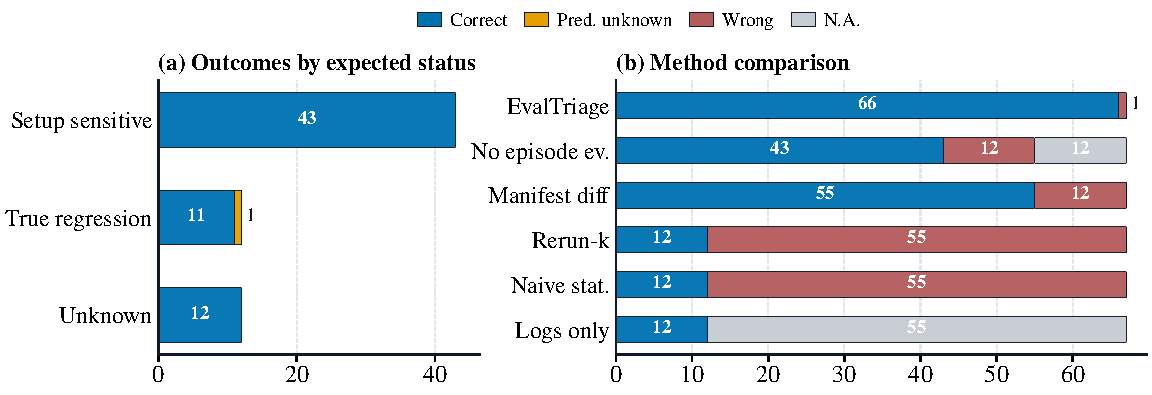
\includegraphics[width=\columnwidth]{figures/rq2_status_overview.pdf}
  \caption{RQ2 status classification: panel (a) shows \sys outcomes by expected status, and panel (b) compares methods by correct, wrong, predicted-unknown, and not-applicable outcomes.}
  \label{fig:rq2-status}
\end{figure}

\subsection{RQ3: Factor Attribution and Abstention}
\label{sub:rq3}

\noindent\textbf{Design.} RQ3 evaluates the central claim of \sys: a deviation diagnosis should connect an observed behavior change to an engineering factor and should abstain when that connection is unsupported. We therefore evaluate completed-rollout and failed-run cases separately. Completed-rollout cases require a thresholded metric or paired-outcome deviation plus replay evidence. Failed-run cases require an execution failure and evidence that the replay or corrected setup recovers execution. Negative calibration cases test the opposite behavior: even if a manifest field differs, \sys should not attribute a factor when no thresholded deviation is detected.

\noindent\textbf{Results.} Table~\ref{tab:paper-results} summarizes the paper-only matrix. Among detected cases, \sys attributes all deviations to the expected factor: 12/12 completed-rollout cases and 4/4 failed-run cases. The combined detected/applicable Top-1 result is therefore 16/16. Under the all-case denominator, the result is 16/20 because the paper-only matrix contains four completed-rollout negative calibration cases where the correct behavior is abstention rather than attribution. The remaining eight negative calibration cases are used only for the robustness/ablation false-attribution denominator. This denominator split is deliberate: detected/applicable Top-1 asks whether \sys identifies the factor when the diagnosis is applicable, while all-case Top-1 keeps abstention cases visible.

\begin{table}[!t]
  \caption{Paper-Only Diagnosis Results}
  \label{tab:paper-results}
  \centering
  \footnotesize
  \renewcommand{\arraystretch}{1.12}
  \begin{tabular}{@{}lrrr@{}}
    \toprule
    Bucket & Detected & Top-1 & All-case \\
    \midrule
    Completed rollout & 75.0\% & 100.0\% & 75.0\% \\
    Failed run & 100.0\% & 100.0\% & 100.0\% \\
    Combined & 80.0\% & 100.0\% & 80.0\% \\
    \bottomrule
  \end{tabular}
\end{table}

\subsection{Ablation and Robustness}
\label{sub:ablation}

\noindent\textbf{Design.} The ablation asks which evidence sources make the attribution reliable. We compare the full method against variants that remove replay evidence, remove episode-level evidence, use manifest differences as a heuristic, use single-run judgment, use a rerun-$k$ style judgment, use a naive statistical gate, or rely on failure-log regexes. These variants are intentionally simple: they represent plausible shortcuts that developers or continuous-integration (CI) systems might use when they do not have factor-directed replay. We recompute the ablation from case artifacts rather than trusting stored baseline summaries, so each method is evaluated under the same artifact contract.

\noindent\textbf{Results.} Table~\ref{tab:ablation} and Figure~\ref{fig:rq3-attribution} summarize the combined robustness ablation. The full method achieves 43/43 detected/applicable Top-1 attribution and 43/55 all-case Top-1, with 0/12 false attributions across the four paper-only and eight robustness-only negative calibration cases. Removing replay lowers detected Top-1 to 38/43. Removing episode evidence lowers the applicable denominator because several completed-rollout cases require paired outcome evidence. The manifest-only heuristic reaches 35/43 detected Top-1 but falsely attributes all 12 negative calibration cases, showing why manifest differences should be treated as suspects rather than causal explanations. The figure also shows the failure anatomy: no-replay misses concentrate in wrong Top-1 factors, no-episode-evidence misses concentrate in no-top-factor outcomes and failed-run non-applicability, and logs-only regex is applicable only to failed runs.

\begin{table}[!t]
  \caption{Combined Ablation Results}
  \label{tab:ablation}
  \centering
  \scriptsize
  \renewcommand{\arraystretch}{1.10}
  \begin{tabular}{@{}lrrr@{}}
    \toprule
    Method & Det. Top-1 & All-case & False attr. \\
    \midrule
    \sys full & 100.0\% & 78.2\% & 0.0\% \\
    No replay & 88.4\% & 69.1\% & 0.0\% \\
    No episode ev. & 64.5\% & 36.4\% & 0.0\% \\
    Manifest diff & 81.4\% & 63.6\% & 100.0\% \\
    Logs only & 100.0\% & 21.8\% & 0.0\% \\
    \bottomrule
  \end{tabular}
\end{table}

\begin{figure}[t]
  \centering
  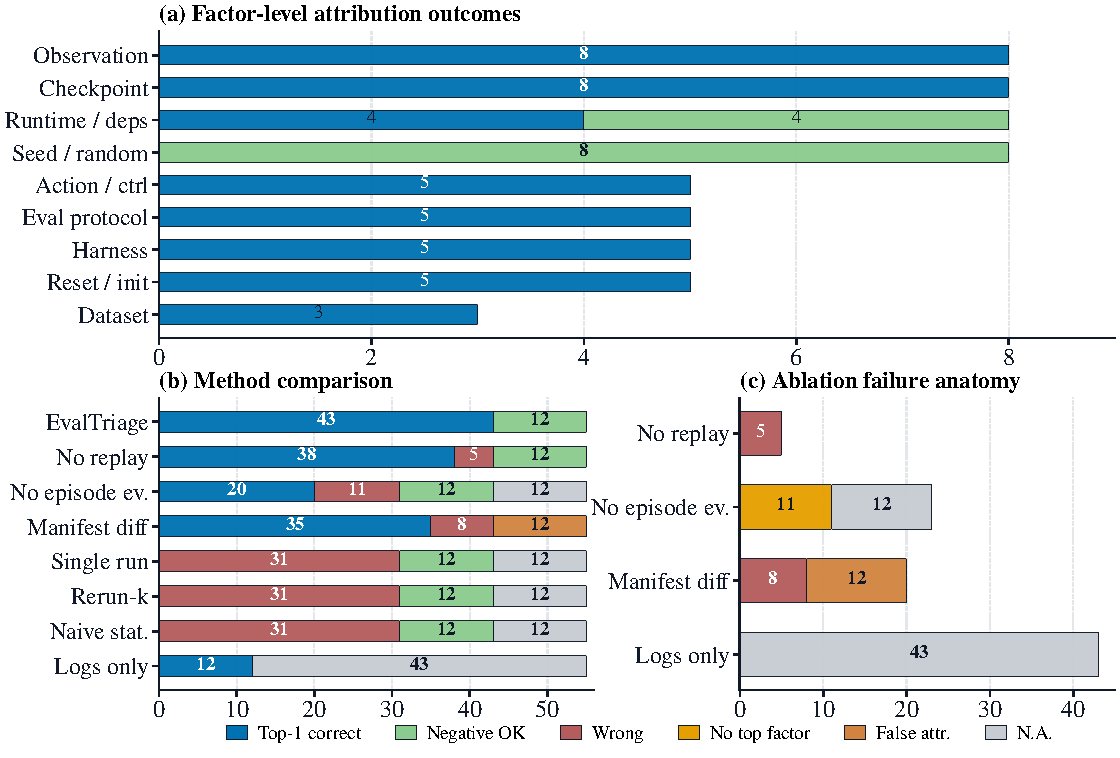
\includegraphics[width=\columnwidth]{figures/rq3_factor_attribution_overview.pdf}
  \caption{RQ3 factor attribution and ablation: panel (a) reports factor-level attribution outcomes, panel (b) compares methods, and panel (c) breaks down ablation failures into wrong, no-top-factor, false-attribution, and not-applicable outcomes.}
  \label{fig:rq3-attribution}
\end{figure}

\subsection{RQ4: Diagnosis Cost}
\label{sub:rq4}

\noindent\textbf{Design.} RQ4 measures the cost of obtaining diagnosis evidence. We report the observed graphics processing unit (GPU) cost of paper-only cases and, for completed-positive cases, the replay workload needed to collect factor-directed evidence. These values are diagnosis-cost measurements for the current artifact pipeline, not claims about model training cost. The key comparison is between affected-task replay, a full single replay, and a blind rerun-$k$ baseline with $k=3$.

\begin{figure}[t]
  \centering
  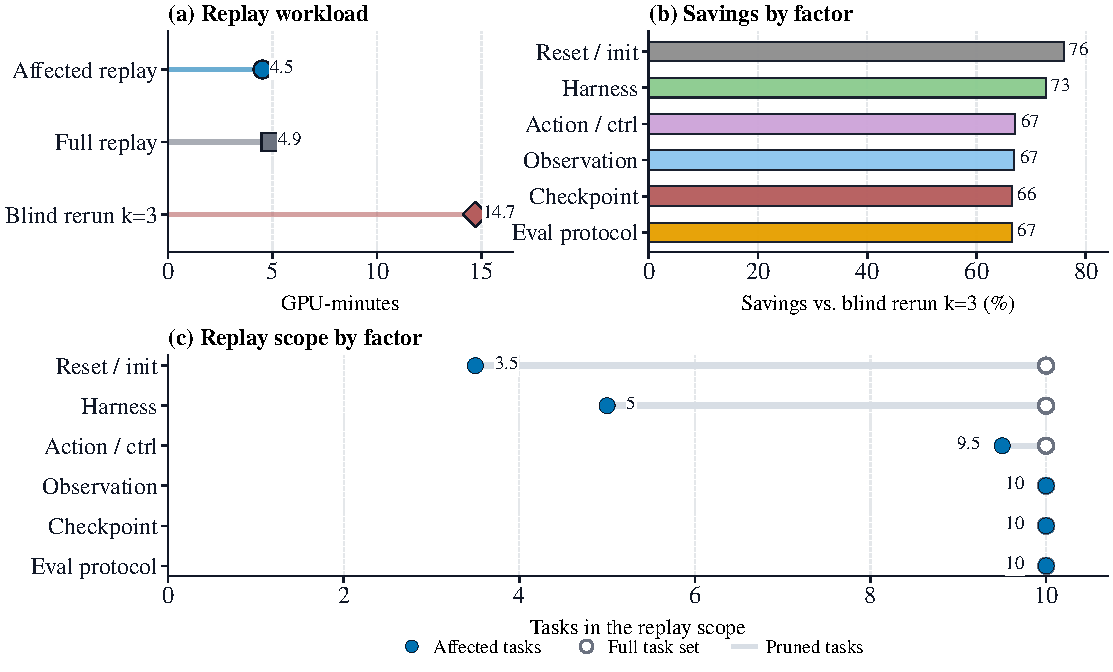
\includegraphics[width=\columnwidth]{figures/rq4_cost_overview.pdf}
  \caption{RQ4 diagnosis cost: panel (a) compares replay workloads, panel (b) reports savings over blind rerun-$k$, and panel (c) shows how affected-task replay prunes the task scope by factor.}
  \label{fig:rq4-cost}
\end{figure}

\noindent\textbf{Results.} Table~\ref{tab:cost} summarizes paper-only cost measurements, and Figure~\ref{fig:rq4-cost} shows the replay-workload comparison. Completed-positive cases average 15.41 observed GPU-minutes and 22.89 wall-clock minutes per case. Their measured affected-task replay averages 4.52 GPU-minutes, close to a full single replay when the affected task set spans most tasks, but far below the 14.71 GPU-minutes of a blind rerun-$k$ baseline. Savings against blind rerun-$k$ range from 66\% to 76\% across factor buckets. The largest replay-scope reductions occur for reset/initial-state and harness cases, where the affected task sets average 3.5 and 5.0 tasks out of 10 respectively. Failed-run cases are cheaper to observe on average because the current run fails early, but they still require recovery evidence before attribution.

\begin{table}[!t]
  \caption{Paper-Only Diagnosis Cost}
  \label{tab:cost}
  \centering
  \scriptsize
  \renewcommand{\arraystretch}{1.10}
  \begin{tabular}{@{}lrrrr@{}}
    \toprule
    Bucket & N & Obs. GPU & Obs. wall & Aff. GPU \\
    \midrule
    Comp. positive & 12 & 15.41 & 22.89 & 4.52 \\
    Comp. negative & 4 & 14.79 & 19.95 & -- \\
    Failed run & 4 & 5.22 & 8.05 & -- \\
    All paper & 20 & 13.25 & 19.34 & -- \\
    \bottomrule
  \end{tabular}
  \vspace{1pt}
  \parbox{0.96\columnwidth}{\scriptsize GPU/wall values are minutes. Aff. GPU is measured for the 12 completed-positive cases where affected-task replay is meaningful.}
\end{table}

\section{Discussion}
\label{sec:discussion-threats}

\subsection{Why Negative Calibration Matters}

Manifest differences are not sufficient evidence for attribution. A runtime version, seed, or configuration field may differ without causing a thresholded deviation; developers may also change logging, task order, or dependency metadata without changing measured behavior. Negative calibration cases therefore test whether \sys treats such differences as suspects rather than causes unless behavioral deviation and replay evidence support them.

\subsection{Completed Rollouts and Failed Runs}

Completed rollouts and failed runs expose different evidence, so we report them separately. A completed-rollout recovery says that the policy can recover baseline behavior when a factor is controlled; a failed-run recovery says that the evaluation pipeline can return to an executable state. Both support triage, but they lead to different actions: inspecting benchmark semantics or adapters in the former case, and fixing environment setup, missing fields, or compatibility assumptions in the latter.

\subsection{What \sys Does Not Decide}

\sys does not decide whether the current policy is better or worse than the baseline, or whether a setup-sensitive change is desirable. A protocol change may be intentional, a controller-interface change may be part of a migration, and a dependency update may be necessary. \sys only supplies evidence about why the evaluation changed; developers still decide whether to accept, document, revert, pin, or request more replay evidence.

\subsection{Implications for Evaluation Maintenance}

\sys is intended to sit between ordinary benchmark execution and human review. A continuous-integration (CI) job or release script can run the evaluation, produce the artifact contract, and invoke the diagnosis layer only when the current result deviates from a baseline. The output should then be read as a triage report rather than as an automatic merge decision: an action-interface diagnosis points toward adapter semantics, a checkpoint/config diagnosis points toward processor statistics or normalization state, and a failed-run dataset diagnosis says that model quality should not be interpreted until the data contract is repaired.

This changes the developer workflow from asking ``did the score drop?'' to asking ``what evidence explains the drop, and what evidence is still missing?'' Aggregate success rates are not enough once a deviation appears; developers need task-level outcomes, paired episode records, manifest fields, failure stages, and replay provenance. The artifact contract in \sys is deliberately small because the goal is not to replace experiment trackers, but to preserve the minimal evidence needed for benchmark-maintenance debugging.

\section{Threats to Validity}

\noindent\textbf{Internal validity.} Threats include threshold choices, replay budgets, controlled-factor correctness, and oracle leakage. We mitigate these threats by separating negative calibration, ablations, and robustness cases from the paper-only matrix, and keeping expected-factor labels outside diagnosis inputs. Construct validity concerns whether success-rate drops, failed-run status, and paired episode shifts capture developer-facing deviations; we derive these symptoms from GitHub issue and pull-request evidence.

\noindent\textbf{Empirical-study validity.} The RQ1 study is a mining and single-annotator manual-classification study over public maintenance records, not a statistically sampled prevalence study. The 473 records therefore support the existence and diversity of the diagnosis problem, but should not be read as exact population rates. We mitigate this by freezing the JSONL records, retaining evidence quotes and URLs, and computing all RQ1 tables deterministically from the frozen input.

\noindent\textbf{External validity.} Threats include the focus on LeRobot+LIBERO and one primary policy. The controlled cases are real LeRobot+LIBERO evaluations and failed-run artifacts, but still controlled instances rather than naturally occurring histories from many stacks. EvalTriage's operators may need extension for other simulators, robot embodiments, or hardware-in-the-loop deployments; we present these results as artifact-level causal validation, while the GitHub study motivates the broader factor vocabulary.

\noindent\textbf{Flaky-status evidence.} Our RQ2 evidence does not support a strong flaky-classification claim. The flaky probes did not produce thresholded repeated-run instability, so the main status result excludes them and reports setup-sensitive, likely true-regression, and unknown cases instead. Future work should evaluate flaky status on naturally unstable benchmark histories or larger repeated-run campaigns.

\section{Related Work}
\label{sec:related-work}

\noindent\textbf{Regression and machine-learning testing.}
Regression-testing work studies test selection, prioritization, and reruns after software changes~\cite{yoo2012regression}, while flaky-test work detects and root-causes tests whose outcomes vary without code changes~\cite{luo2014flaky,bell2018deflaker,lam2019root}. Machine-learning (ML) testing work proposes metamorphic, white-box, coverage-guided, and criteria-based techniques for finding model errors~\cite{xie2011metamorphic,pei2017deepxplore}, with surveys covering test generation, oracle design, robustness, and debugging~\cite{zhang2022mltesting,braiek2020testing}. \sys is complementary: it does not generate tests or model coverage criteria, but diagnoses why an already-observed embodied-AI evaluation changed.

\noindent\textbf{AI pipelines and provenance.}
Empirical and practice-oriented work shows that AI-system behavior depends on data, configuration, infrastructure, APIs, and hidden dependencies~\cite{zhang2018tensorflowbugs,humbatova2020faults,amershi2019se4ml,martinezfernandez2022survey,breck2017mltest,sculley2015debt}. ML lifecycle and provenance systems record metadata, artifacts, metrics, workflow state, and data-quality checks~\cite{baylor2017tfx,zaharia2018mlflow,schelter2018deequ,moreau2011opm}. \sys uses provenance as a starting point, but adds causal discipline: a manifest difference becomes a diagnosis only when behavioral or failure-recovery evidence supports it.

\noindent\textbf{Embodied-AI tasks and benchmarks.}
Embodied-AI and robot-learning benchmarks define not only task goals, but also simulators, assets, observations, controllers, resets, language conditions, demonstrations, and success metrics. Habitat targets embodied navigation and interaction in photorealistic 3D environments~\cite{savva2019habitat}; Meta-World, RLBench, robosuite, ManiSkill2, and LIBERO cover different forms of robotic manipulation, multi-task learning, generalizable manipulation skills, and knowledge transfer~\cite{yu2020metaworld,james2020rlbench,zhu2020robosuite,gu2023maniskill2,liu2023libero}; CALVIN emphasizes long-horizon language-conditioned manipulation~\cite{mees2022calvin}; and LeRobot provides a reusable open-source robot-learning library and evaluation interface~\cite{lerobot2026}. These benchmarks are essential for measuring embodied policies, but their richness also creates many engineering boundaries where evaluation behavior can change. \sys does not propose a new task suite; it diagnoses deviations that arise when such suites and harnesses are maintained as software.

Existing benchmark work primarily defines tasks, datasets, simulators, and reporting protocols so that policies can be compared. \sys addresses a later maintenance question: after a benchmark and policy already exist, what should developers do when the measured outcome changes? The answer cannot be read from the aggregate score alone because the score is downstream of simulator state, reset choices, sensor preprocessing, action semantics, and metric definitions. Treating those components as diagnosable factors is the main difference between \sys and benchmark design work.

\noindent\textbf{Embodied-AI reproducibility.}
Reinforcement-learning (RL) and robot-learning results are sensitive to benchmark design, implementation choices, seeds, simulators, and reporting practices~\cite{duan2016benchmarking,henderson2018drlmatters,engstrom2020implementation,pineau2021reproducibility,patterson2024empirical}. The Arcade Learning Environment (ALE) and MuJoCo show the long-standing role of benchmark protocol and simulator semantics in RL evaluation~\cite{machado2018ale,todorov2012mujoco}. EvalTriage addresses a different layer of reproducibility: once a benchmark result changes, it asks which evaluation factor is supported by artifacts and replay evidence, and when evidence is too weak to attribute.

\section{Conclusion}
\label{sec:conclusion}

This paper defines embodied AI evaluation deviation diagnosis as a software engineering problem and presents \sys, a manifest- and replay-based approach for classifying deviations, ranking engineering factors, and abstaining when evidence is insufficient. The empirical study shows that real projects contain diverse deviation symptoms and many under-specified factor reports, while the LeRobot+LIBERO evaluation shows that factor-directed replay can convert metric changes and failed executions into developer-facing diagnoses. Negative calibration, ablation, robustness, and cost results further show why replay evidence, conservative abstention, and targeted replay matter. The broader lesson is that embodied-AI benchmark results should be treated as outputs of an evaluation pipeline, not as policy-only measurements: a score change becomes actionable only when developers can connect it to manifest, episode-level, failure, and replay evidence.

\section*{Data Availability}

An anonymized artifact package is available at \href{https://anonymous.4open.science/r/evaltriage-artifact-2610/}{\nolinkurl{anonymous.4open.science/r/evaltriage-artifact-2610/}}. The package contains the frozen empirical-study records, case configurations, derived metrics, diagnosis artifacts, ablation outputs, cost metrics, and figure/table scripts needed to audit the paper's main results. Large policy checkpoints, datasets, simulator assets, caches, and raw videos are documented but not bundled because of storage and redistribution constraints.


\ifshowrefs
  \clearpage
  \bibliographystyle{IEEEtran}
  \bibliography{refs}
\fi

\end{document}
